% !TEX root = ../main.tex
\chapter{IoT Brain} \label{ch:framework}

This chapter is going to give some informations about the design choice taken while implementing the approaches in \textbf{\autoref{ch:model}} and \textbf{\autoref{ch:diagnosis}}.
Implementation efforts were aimed at providing a further degree of scalability to the approach and leveraging cloud based technologies as well as reducing the technicality of the involved resource.
It will be presented a use case that shows the % TODO explain why this framework can help in spreading a EMS
\section{Fully integrated BMS}
Previous chapters defined a possible approach for diagnosing smart buildings, developed by IBM Research and it has been shown that such a method works as expected.
However such instruments needs to be integrated in a broader panorama of services that should be present in a Smart Building. Defining the term Smart Building is a challenging task and various organizations adopt their own definition. % TODO add definitions
What emerges is that a smart building has to be able to perceive the context it is in, being aware of its status and its occupants. Another key concept it is its ability to react, and adapt, autonoumsly to changes in the environment, possibly predicting and optimizing its behaviour in order to optimize occupants comfort and energy consumption.
IoT devices provide the context for a Smart Building. Commercial buildings are costantly monitored by IoT smart sensors and meters that provide a huge amount of data. Those data are stored and processed to extract useful information on the state of the building. % TODO chart how many sensors
Analytics provide the means that the building use to interpret the context and react in a correct way. For example, let a fault occour at a Fan Coil Unit (FCU) in a room. A smart building should be able to detect it, diagnose it, eventually issue a repair request to the manteinance service with a description of the fault. Then, upon arrival of the mainteinance worker, the building should be able to guide said worker through the building itself towards the location of the fault.

\section{Requirements}
In a Smart Building context it is important to understand what are the main goals that are to be achived by the deployment of such a system. What emerged from this thesis work is that a Smart Building IT infrastructure needs to be build upon a scalable framework that provides a platform for easy and fast analytics deployement. There's a need of a middleware that provide every top level application with a common ground that abstract the physical sensors so that the whole system is integrated and top layer components are able to exchange informations. % example integration of weather data etc.
This middleware is born from the Semantic Web concept of ontology (see \autoref{ch:semantic_web}) and of semantic reasoning. What is different here is that the scope is note the same. Semantic Web technologies have their focus on massive amount of diverse data that comes from different sources and their goal is somewhat to unify them, a single ontology won't suffice to capture that complexity and therefore highly complex solutions have been developed (OWL). In that context it is of utmost importance the standarization of the approaches and a strict formality in their representation. In the context of Smart Buildings these focus are shifted and requirements become somewhat more lax. Building's data are sensible ans are not supposed to be exchanged outside of the scope of a single organization (a company, a university, etc.), additionaly, since the goal of this framework is to manage a building, the concepts involved are little in numbers and simpler in structure than those involved in the Semantic Web. \textcite{brick_schema} showed how a little number of concepts and relationships (see \autoref{fig:brick_schema}) is required for capturing the complexity of a building. Orthogonal to this, another simple ontology SSNO and its extension (see \autoref{subsec:ssn}), developed by IBM Research, suffice for capturing the complecity of physical interaction between buildings assets, as seen in \autoref{fig:extended_ssno}.
On top of this, it is important to identify and focus on the potential users of such a system. Those users are both those who benefit from the deployed analytics and those who are going to develop those analytics. It is important to note that none of those users is required to have a deep computer science background of any sort, still they are the ones with most interest in a smart building management system. The system should aim at providing those users the most straightforward default way to interact with the system, trough high-level languages and possibily human language interfaces (see ) but still allows for low level interaction where needed. To sum it up:
\begin{itemize}
  \item Easy development tools
  \item High level scripting languages
  \item Semantic capabilities to enable integration
  \item Scalable backend
\end{itemize}

\section{Knowledge Inference Technology for IoT}
Knowledge Inference Technology for IoT (KITT) is a layered framework that provide an API to model, manage and reason on the semantic knowledge of IoT Systems. It has been developed by IBM Research and expanded with further capabilities as the core of this thesis. It is designed to meet the requirements outlined in the previous section and to provide a service for integrated deployment of analytics in IoT contexts.
KITT adopt a layered approach as seen in \autoref{fig:kitt}.
\begin{figure}
  \centering
  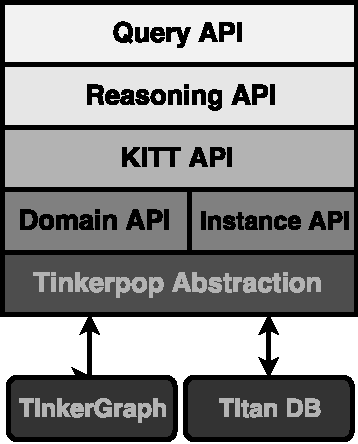
\includegraphics{kitt.pdf}
  \caption{KITT internal structure}
  \label{fig:kitt}
\end{figure}
Each of these layers implements different functionalities that will be detailed just below

\subsection{TinkerPop abstraction layer}
This layer is strictly related to the low level implementation of the graph on the physical store. What is important to note is the choice of representation of the underlying RDF graph that is the base of the semantic approach. Altough many RDF stores and semantic databases are available, the choice made verted towards a graph Data Base (DB) implementation of said RDF graph. The main reason is to be searched in the scalability needs of the project and the scope of it. What has been developed is an integrated semantic framework for Smart Buildings and not a multipurpose layered semantic engine.
\paragraph{GraphDB vs. RDFStore}
It is important to note that the word semantic doesn't necessarly mean RDF. When talking about semantic it is intended a way to give a meaning to otherwise unmeaningful data so that more complex operations can be performed, thanks to the abstraction that such additional knowledge provide. It has been said in \autoref{subsec:rdf} that RDF is a way to store triples, and that those triples represent a graph. Ontologies, then, are still triples that makes use of some well known concepts and relationships (e.g Class and subClassOf) to give a meaning to RDF triples. It follows that RDF data, both ground truth and ontologies, can be safely stored in a graphDB. There are also some advantages in using a graph representation. For instance, graph DB implements the so called Labeled Property Graph (LPG) whose main advantage is that of storing vertexes and labels that can have an internal structure. In practice, this allows for the chance of storing additional data, whose semantic description is not essential, without complicating the ontology. IT is possible to trace the root of this in the
\paragraph{Apache TinkerPop}
The TinkerPop abstraction layer has been developed in order to abstract the underline storing engine and provide vendor indipendance. This layer provide a series of methods that can be used by upper layers to directly operate on the graph without worrying about the underline technology. Changing the graphDB engine just requires the right implementation of the abstraction layer without further modification of the upper layers. Apache TinkerPop itself  an open source, vendor-agnostic, graph computing framework distributed under the commercial friendly Apache2 license.

\subsection{Domain API and Instance API}
These layers both work upon the TinkerPop Abstraction layer as they are the main component involved while building the model of a building. The domain API acts when defining the taxonomy of a domain. For example, whenever it is needed to express that a new concept exists, like a Room is a subClassOf a Location, that is Domain API duty. The Instance API is, instead, in charge of the creation of new facts, that are the specific knowledge about a system. This API is the one responsible, for example, of the creation of new instances, such that Room0408 is a instance of the concept Room. In \autoref{fig:dom_inst_api} it is detailed which API an instance and a concept are going through when they are created in the graph.
\begin{figure}
  \centering
  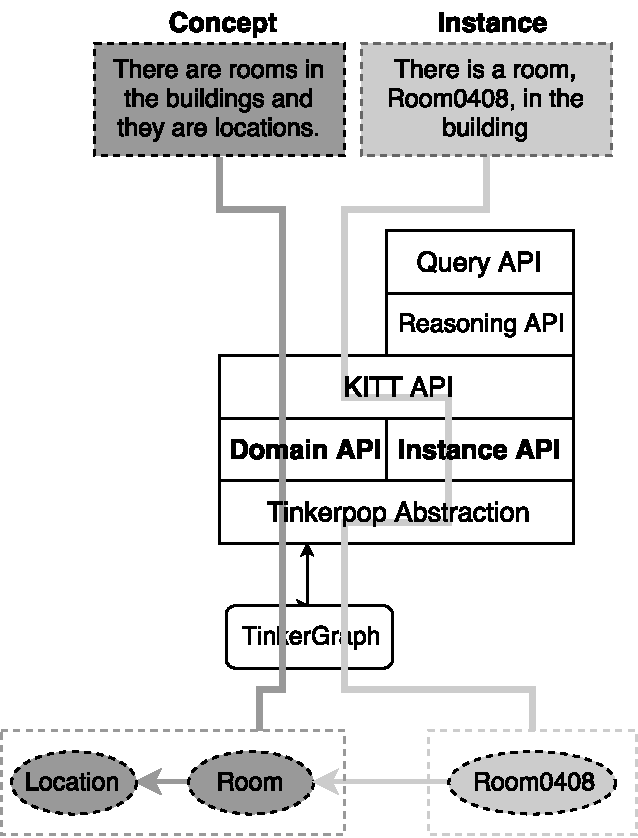
\includegraphics[width=.4\textwidth]{conc_inst_api.pdf}
  \caption{Usage of the Domain and Instance API}
  \label{fig:dom_inst_api}
\end{figure}

\subsection{KITT API}
KITT API is the middle ground between lower layers and upper layers. At this point of the stack everything is abstract enough so that the main focus shift towards the user of the system, be it human or an application. KITT API provide high level endpoints that allow for interactions with the lower level domain and instance endopoints through high level text base format (JSON, KITT scripting).

\paragraph{KITT scripting}
KITT scripting language is a way for the end user to inject in the system a whole model in a straightforward way. A end user should be able to load a whole model without worrying about implementation details or technical aspects of reasoning and ontology modelling. This lead to the development of a simplified scripting language for ontology creation, that is simple yet expressive enough for implementing the needed relationships of Brick (\autoref{subsec:brick}) and SSN (\autoref{subsec:ssn}) ontologies. It is based on the following assumptions:
\begin{itemize}
  \item Domain concepts and relationships are structured in a taxonomy and so are disjointed
  \item Relationships can be established between concepts or between instances
  \item Relationships between concepts and instances are only the instantiation ones
  \item Instances have to be instantiated from the defined model.
\end{itemize}
Thanks to these assumptions the scripting language can define a full model in a human readable text format. This format separates the on
tology definition from the instances definition.

\subsection{Reasoning API}
Whenever reasoning is involved, it is intended as the capability of inferring new knowledge about the system given previous asserted facts and an ontology. The main duty of the reasoning engine in this project is that of applying knowledge about general physics to the given model. The second one is it's capacity of answering complex query that the KITT API level can't natively handle. Therefore KITT reasoning language describe an union of production rules languages like SWRL and query languages like SPARQL.
\paragraph{KITT reasoning language}
The reasoning language developed borrowed syntax from classic rule languages like SWRL, yet it needed to expose methods useful to explicit complex query and path traversal. A KITT rule is expressed as a form of entailment \[body\Rightarrow head\] where $body$ and $head$ are both expressed in conjunctive form, so that a rule assume the form \[A_1\land\ldots\land A_n\Rightarrow B_1\land\ldots\land B_m\] where $A_i$ and $B_j$ are either statements about, or relationships between, facts (see \autoref{eq:rule_facts_only}).
\begin{equation}
\label{eq:rule_facts_only}
Room0408\land Temp0408\Rightarrow hasProperty(Room0408, Temp0408)
\end{equation}
That means that wether the condition in the body holds, the condition on the left must hold too. This characteristic, typical of production rules, is used to entail new knowledge according to domain expertise. When coupled with the concept of variable, rules becomes a powerful tool to enforce knowledge on a knowledge base. Thanks to variable, rules can be wrote refering to concepts, that in turn are set of instances; this allows for the encoding of domain expertise into procedural rules. For example, a human expert would not say something as in \ref{eq:rule_facts_multiple}
\begin{equation}
\label{eq:rule_facts_multiple}
\begin{gathered}
Room0408\Rightarrow hasProperty(Room0408, Temp0408)\land Temp0408\\
Room709\Rightarrow hasProperty(Room709, Temp709)\land Temp709\\
\dots
\end{gathered}
\end{equation}
but would instead say ``Every room has an internal temperature''; from this sentence it emerge that there exist a concept of room, a concept of internal temperature and that this concepts are related. Introducing variables it becomes a rule as in \autoref{eq:simple_prod_rule}
\begin{equation}
\label{eq:simple_prod_rule}
Room(x)\Rightarrow Temperature(y)\land hasProperty(x,y)
\end{equation}
where $x$ and $y$ are variable that can be bound to any given facts in the instance model; if  the variables appears on the right-hand side of the rule and can't be bound to any given fact in the knowledge base, they are created so that the entailment is satisfied. It is to note that this behaviour is usually prohibithed by existing reasoners due to the fact that it remove the decidability property from the ruleset.
That is, if in a production ruleset a variable appears in the right-hand side of a rule whilst not appearing in the left-hand side of
A less traditional ways to use this kind of rules is for the evaluation of property chains. Property chains, in the context of physical modelling and diagnosis represents important knowledge (see \autoref{sec:potential_causes}) and the ability to traverse them is essential for reasoning in such environments. An ad-hoc operator has been introduced so that such traversal are possible
\begin{verbatim}
 _CHAIN({R(dir),R(dir),...}, start, end)[condition]
\end{verbatim}
where \verb|R| is a relationship in the ontology, \verb|dir| $\in$ \verb|[^,v]| tells wether the relationship to chase is an incoming or outcoming one and when are combined as in \verb|{R(dir)...}| they specify a pattern to match; \verb|start| identify a known variable in the head of a rule and so is \verb|end|, respectively identifying the first and last instances of the chain, \verb|condition| is either a number specifying the max number of pattern matching to perform before stopping, a condition the \verb|end| variable needs to uphold in order to stop the recursion or both. Such function is visible in \autoref{fig:property_chain_rule}. In the case that a cycle is identified during the traversal it is natively dealt with using standard cycles detection algorithms.
\begin{figure}
  \centering
  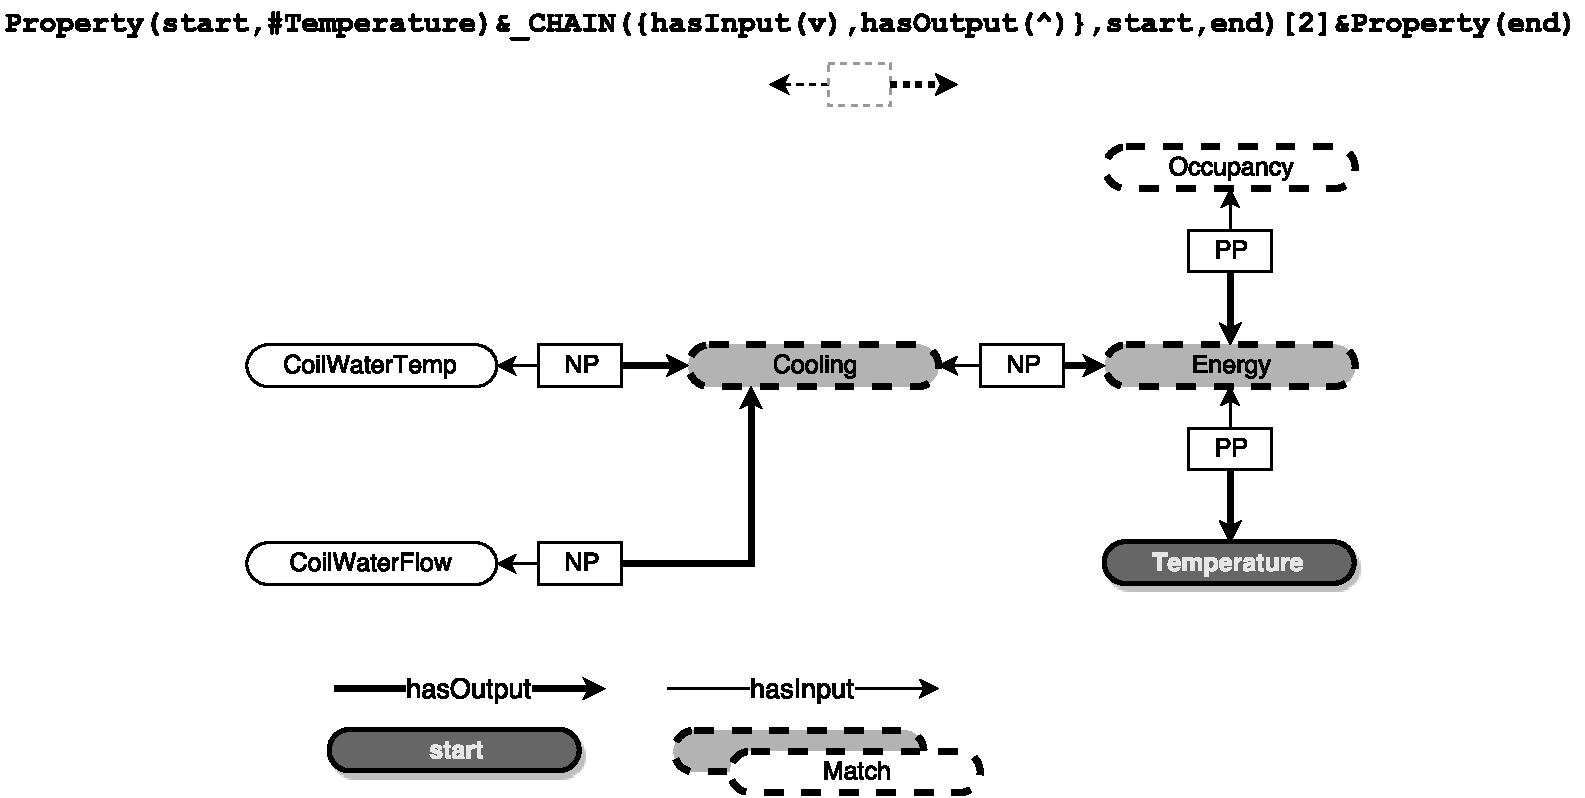
\includegraphics[width=.8\textwidth]{property_chain_rule.pdf}
  \caption{Property chain in a rule}
  \label{fig:property_chain_rule}
\end{figure}

